\subsection{Aufgabe 1: Zeitmessung bei Fibonacci-Implementationen}
Sie erhalten als Vorgabe die beiden Dateien fiboit.c und fiborek.c. Sie beinhalten eine iterative Implementation
der Fibonacci-Zahlen, respektive eine rekursive Implementation, jeweils in der Programmiersprache
C.
\begin{enumerate}
  \item Implementieren Sie die beiden Programme je in C++ (sie müssen nicht objektorientiert sein).
  \item Sie haben gesehen, dass die rekursive Implementation mit der Fakultät wächst. Verifizieren Sie die Theorie, indem Sie Zeitmessungen für die Berechnung vornehmen.
\end{enumerate}

\textbf{Hinweis zu den Zeitmessungen:}

Mit einfachen Mitteln ist eine genaue absolute Zeitmessung nicht durchführbar. Für unsere Zwecke genügt
hier eine relative Zeitmessung, die genügend genau ist. Wählen Sie eine der folgenden Varianten:

Variante 1: Messung der Standardzeit

Die Funktion \texttt{clock()} aus \texttt{<ctime>} liefert die abgelaufene CPU-Zeit in Clockticks seit Programmstart. Wenn
diese Grösse durch \texttt{CLOCKS\_PER\_SEC} geteilt wird, erhält man eine Zeit in Sekunden.
\begin{lstlisting}[language=C++, style=C++]
#include <ctime>
clock_t start = clock();
// do something
clock_t end = clock();
cout << "Ticks: " << end-start << endl;
cout << "Time: " << static_cast<double>(end-start) / CLOCKS_PER_SEC << " sec" << endl;
\end{lstlisting}

Variante 2: Native Zeitmessung von Linux
\begin{lstlisting}[language=C++, style=C++]
#include <sys/resource.h>
#include <sys/types.h>
rusage tp;
double start; // Startzeit in Millisekunden
double end; // Endzeit
getrusage(RUSAGE_SELF, &tp);
start = static_cast<double>(tp.ru_utime.tv_sec) +
        static_cast<double>(tp.ru_utime.tv_usec)/1E6;
// do something
getrusage(RUSAGE_SELF, &tp);
end = static_cast<double>(tp.ru_utime.tv_sec) +
      static_cast<double>(tp.ru_utime.tv_usec)/1E6;
cout << "Dauer: " << end-start << " sec" << endl;
\end{lstlisting}

\subsubsection{Lösung}

\large{Iterativ + Linux Zeitmessung}
\lstinputlisting[language=C++, style=C++, multicols=2]{900-Praktika/prak03/Loesung/FiboItWatch/fiboit.cpp}

\large{Rekursiv + \texttt{clock()} Zeitmessung}
\lstinputlisting[language=C++, style=C++, multicols=2]{900-Praktika/prak03/Loesung/FiboRekWatch/fiborek.cpp}

\large{Rekursiv + Linux Zeitmessung}
\lstinputlisting[language=C++, style=C++, multicols=2]{900-Praktika/prak03/Loesung/FiboRekWatchLinux/fiborek.cpp}

\subsection{Aufgabe 2: Klasse für Stoppuhr}
Implementieren Sie eine Klasse \texttt{StopWatch}, die sich bei der Gründung eines Objekts die Zeit merkt. Bei
jedem Aufruf der Methode \texttt{elapsed()} wird die bis dahin abgelaufene Zeit in Sekunden zurückgegeben.
Beispiel:

\begin{lstlisting}[language=C++, style=C++]
StopWatch t; // starts stopwatch
double d = t.elapsed();
\end{lstlisting}

\subsubsection{Lösung}

\lstinputlisting[language=C++, style=C++, multicols=2]{900-Praktika/prak03/Loesung/StopWatch/src/StopWatch.h}
\noindent\makebox[\linewidth]{\rule{\paperwidth}{0.4pt}}
\lstinputlisting[language=C++, style=C++, multicols=2]{900-Praktika/prak03/Loesung/StopWatch/src/StopWatch.cpp}
\noindent\makebox[\linewidth]{\rule{\paperwidth}{0.4pt}}
\lstinputlisting[language=C++, style=C++, multicols=2]{900-Praktika/prak03/Loesung/StopWatch/src/StopWatchTest.cpp}
\twocolumn

\subsection{Aufgabe 3: Komplexität}


Es gilt die Annahme, dass ein gewisses Programm jeden Abend exakt eine Stunde Rechenzeit bekommt.
Sie haben herausgefunden, dass das Programm $n=1'000'000$ Datensätze verarbeiten kann. Nun wird ein
neuer Rechner angeschafft, der 100 Mal schneller als der alte ist.
Wie viele Datensätze kann Ihr Programm nun in einer Stunde verarbeiten, wenn wir die folgende Zeitkomplexität
mit den Konstanten $k_i$ annehmen?

\begin{enumerate}
  \item $k_1 \cdot n$
  \item $k_2 \cdot n \cdot \log_{10} n$
  \item $k_3 \cdot n^2$
  \item $k_4 \cdot n^3$
  \item $k_5 \cdot 10^n$
\end{enumerate}

\textbf{Hinweis:}
Verwenden Sie den Ansatz, dass der schnelle Rechner in einer Stunde gleich viel leistet, wie der
langsame in 100 Stunden.

\subsubsection{Lösung}


\textbf{Ansatz:}

\begin{itemize}
  \item Langsamer Rechner: $T(n) = 1 \text{h}$
  \item Schnellerer Rechner : 100 Mal Schneller
  \begin{itemize}
    \item Der schnellere Rechner leistet in 1h gleich viel wie der langsamere in 100 h.
    \begin{enumerate}
      \item $T(n) = 1$ für $n= 10^6$ einsetzen $\Rightarrow$ ergibt $k$;
      \item $T(n)\mathrel{\stackon[1pt]{$=$}{$\scriptstyle!$}} 100 $ setzen mit unter (1.) ermitteltem $k$;
      \item nach $n$ auflösen
        \end{enumerate}
  \end{itemize}
\end{itemize}

\noindent
\textbf{a)}

\medskip

$$ k_1 \cdot 10^6 = 1 \Longrightarrow k_1 = \underline{10^{-6}}$$
$$ k_1 \cdot n = 100 \Longrightarrow n = \frac{1}{k} \cdot 100 = 10^6 \cdot 100 = \underline{\underline{10^8}}$$

\medskip

\noindent
\textbf{b)}
\medskip

$$ k_2 \cdot 10^6\cdot \log_{10} 10^6 = 1$$
$$\Rightarrow k_2 \cdot 10^6 \cdot 6 = 1 \Rightarrow k_2 = \frac{1}{6} \cdot \underline{10^-6}$$
$$ \Rightarrow k_2 \cdot n \cdot \log_{10} n = 100$$
$$ \Rightarrow n \cdot \log_{10} n = 6 \cdot 10^8 =: c_2 $$
$$\Rightarrow 10^{n \cdot \log_{10} n} = 10^{c_2}$$
$$\Rightarrow n^n = 10^{c_2} = 10^{6\cdot10^8}$$
\medskip

Diese Gleichung lasst sich nicht geschlossen lösen.

solver: $\underline{\underline{n= 76 127 253}}$

\medskip

\noindent
\textbf{c)}
\medskip

$$ k_3 \cdot (10^6)^2 = 1 $$
$$\Rightarrow k_3 \cdot 10^12 = 1 \Rightarrow k_3 = \underline{10^{-12}}$$
$$k_3 \cdot n^2 = 100$$
$$\Rightarrow \underline{n} = \sqrt{10^{14}} = \underline{\underline{10^7}}$$
\medskip

\noindent
\textbf{d)}
\medskip

$$ k_4\cdot (10^6)^3 = 1$$
$$ \Rightarrow k_4 \cdot 10^{18} =1 \Rightarrow k_4 = \underline{10^{-18}}$$
$$ k_4 \cdot n^3 = 100 \Rightarrow n^3 = 10^{20}$$
$$ \Rightarrow \underline{n} = 10^{\frac{20}{3}} = \underline{\underline{4641588}}$$
\medskip

\noindent
\textbf{e)}
\medskip
\medskip

$$ k_5 \cdot 10^{10^6} = 1 \Rightarrow k_5 = \underline{\frac{1}{10^{10^6}}}$$
$$ k_5 \cdot 10^{n} = 100$$
$$ \Rightarrow 10^n = 100 \cdot  10^{10^6} =  10^{10^6+2}$$
$$ \Rightarrow \underline{n} = 10^{6} + 2 = \underline{\underline{1000002}}$$

\medskip

d.h. mit einem 100 Mal schnelleren Rechner können Sie 2 (!) zusätzliche Datensätze berechnen.


\onecolumn

\subsection{Aufgabe 4: Sortieralgorithmen}
Implementieren Sie einen rekursiven Quicksort-Algorithmus, der für Teildaten mit weniger als $M$ Elementen
zu Insertionsort (Direktes Einfügen) übergeht.

Bestimmen Sie empirisch den optimalen Wert von $M$. Nehmen Sie einen Array mit ungefähr fünf Millionen
zufällig erzeugten Ganzzahlen an und messen Sie, mit welchem $M$ die Sortierung am schnellsten abgearbeitet
wird. Betrachten Sie dabei sowohl das Sortieren der unsortierten als auch der bereits sortierten Liste.



\subsubsection{Lösung}

Mit dem verwendeten Rechner wurde die Listengrösse mit 5 Mio. Elementen des Typs int gewählt. Die Lis-te musste auf dem Heap angelegt werden, beim Einsatz einer Stackvariablen resultierte ein Stackoverflow.

In Abbildung 1 sind die Laufzeitmessungen dargestellt (Execution time in Sekunden). Wenn die Schwelle auf Null gesetzt wird, gibt es keinen Wechsel des Algorithmus, d.h. das ist der reine Quicksort-Algorithmus. Aus den Messungen ist ersichtlich, dass das Sortieren der unsortierten Liste am schnellsten ist, wenn unterhalb einer Listengrösse von ca. 30-80 auf den Insertionsort umgestellt wird (obere Kurve 'Unsorted'). Wenn die Liste bereits sortiert ist, dann schneidet der reine Quicksort nicht schlechter ab (mittlere Kurve 'Sorted'). Auf-grund der Kombination dieser beider Kurven ist es sinnvoll, die Schwelle auf ca. 30 zu setzen.
Die unterste Kurve stellt das Messrauschen, d.h. die Abweichung bei mehreren Messungen, dar bei der Sortierung von unsortierten Listen. Das Messrauschen ist doch recht hoch.

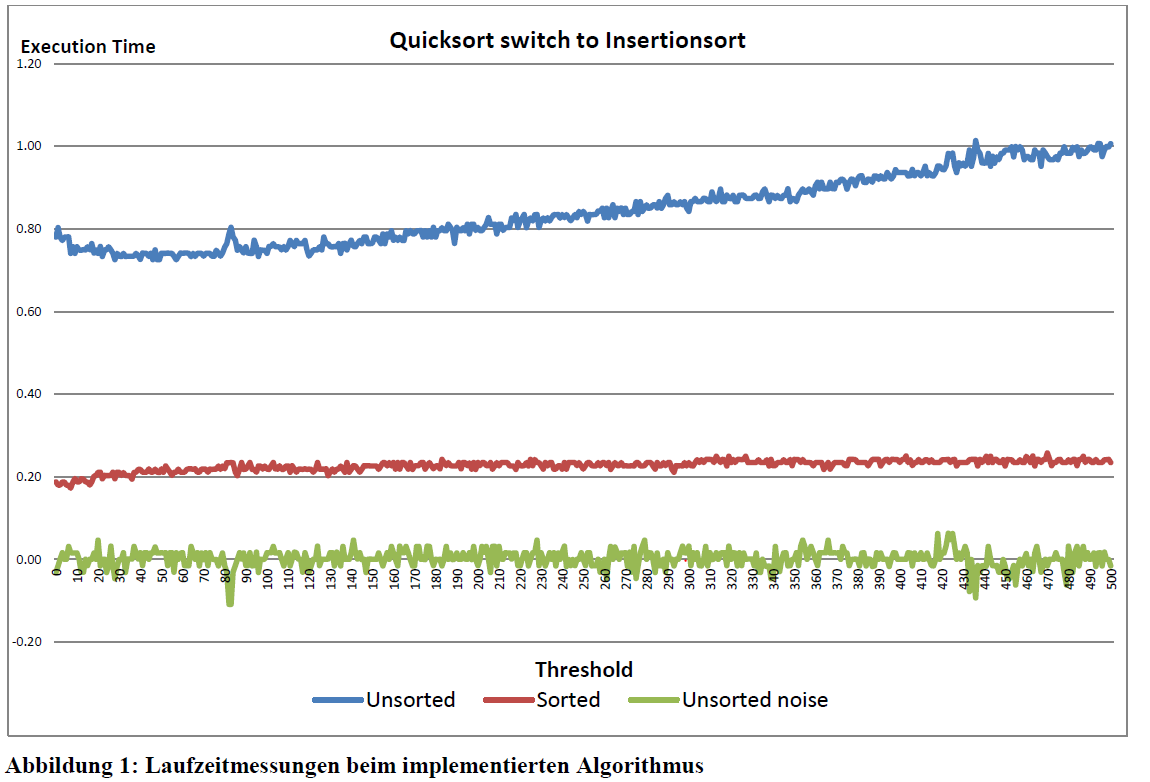
\includegraphics[width=.8\linewidth]{900-Praktika/prak03/pic.PNG}


\lstinputlisting[language=C++, style=C++, multicols=2]{900-Praktika/prak03/Loesung/QuickSortFast/src/List.h}
\noindent\makebox[\linewidth]{\rule{\paperwidth}{0.4pt}}
\lstinputlisting[language=C++, style=C++, multicols=2]{900-Praktika/prak03/Loesung/QuickSortFast/src/List.cpp}
\noindent\makebox[\linewidth]{\rule{\paperwidth}{0.4pt}}
\lstinputlisting[language=C++, style=C++, multicols=2]{900-Praktika/prak03/Loesung/QuickSortFast/src/QuickSortFast.cpp}
\noindent\makebox[\linewidth]{\rule{\paperwidth}{0.4pt}}
\lstinputlisting[language=C++, style=C++, multicols=2]{900-Praktika/prak03/Loesung/QuickSortFast/src/StopWatch.h}
\noindent\makebox[\linewidth]{\rule{\paperwidth}{0.4pt}}
\lstinputlisting[language=C++, style=C++, multicols=2]{900-Praktika/prak03/Loesung/QuickSortFast/src/StopWatch.cpp}
\noindent\makebox[\linewidth]{\rule{\paperwidth}{0.4pt}}
